% !TEX encoding = UTF-8
% !TEX TS-program = pdflatex
% !TEX root = ../Tesi.tex
% !TEX spellcheck = en-EN

%************************************************
\chapter[Experimental Characterization]{Experimental Characterization}
\chaptermark{Experimental}
\label{cap:experimentalcharacterization}
%************************************************

\improvement{Add some propaganda for experimental characterization}



\section{Particle Distribution}
\label{sec:particledistribution}

\improvement{Make a table with the particles diameter distributions of all
materials.}

\section{Angle of Repose (p-p) - Small Scale}
\label{sec:aor}

A sample was deposited on a 20 cm diameter plate with liftable boundary called
static angle of repose (\ac{AoR}) tester, see Fig. \ref{fig:051aorLab}.
Once the particles were in position, the boundary was lifted, allowing some particles to drop. 
Once stabilized, the \ac{AoR} was measured eight times using a digital protractor at different positions of the heap. 
The average of the measurements gave the fourth bulk value.
Note that, since the experiments were performed only for larger-size bulk
solids, the compaction condition in the initial state was not critical to the
final result.\\
\begin{figure}[!htb]
\centering
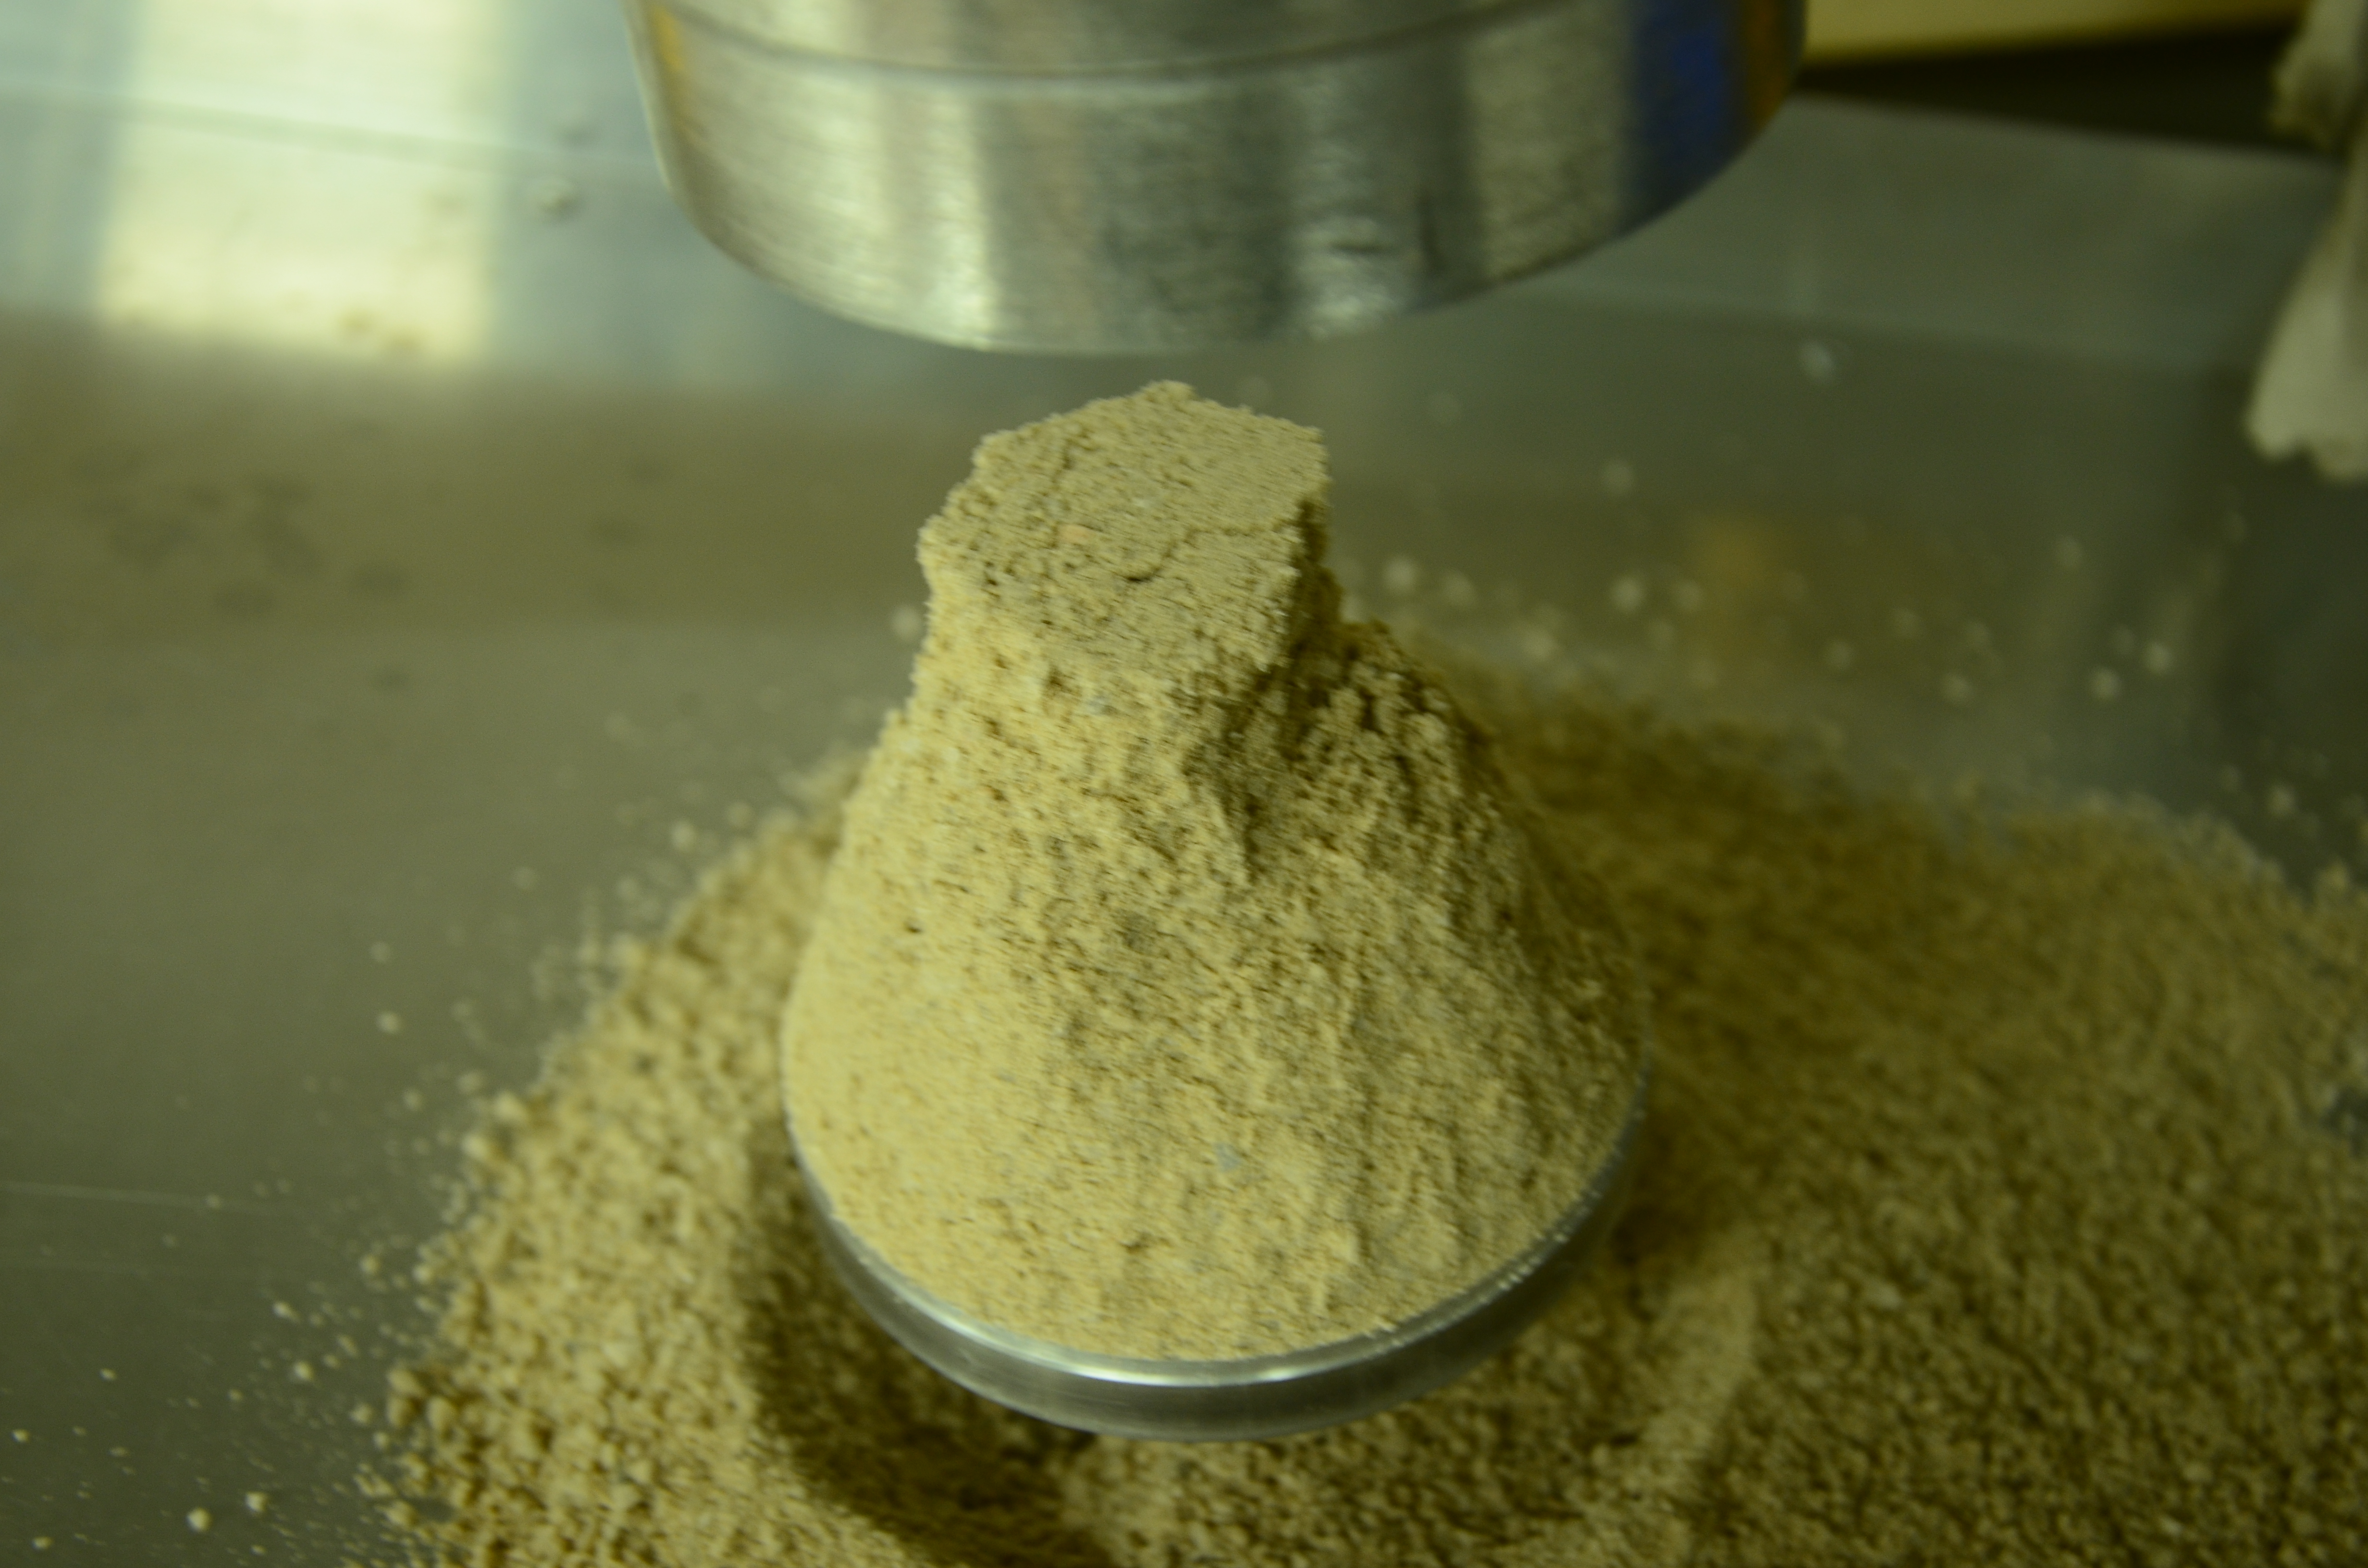
\includegraphics[width=.80\columnwidth]{images/051aorLab}
\caption[AoR]{Drained angle of repose.}
\label{fig:051aorLab}
\end{figure}
\ref{fig:005aor}.\\
\begin{figure}[!htb]
\centering
\includegraphics[width=.80\columnwidth]{images/005aor}
\caption[AoR tester]{Drained angle of repose tester.}
\label{fig:005aor}
\end{figure}

\section{Angle of Repose (p-p) - Large Scale}
\label{sec:aorlargescale}

At the Leoben VAS facility a new rotating double chute was used: 
9 large scale dynamic angle of repose tests were performed. 
\improvement{Evaluate large-small scale AoR relationship.}

\section{Jenike Shear Cell tester}
\label{sec:jsct}
%************************************************

\improvement{Write something about JSCT (simplified version of RSCT, or
viceversa).}
Fig. \ref{fig:052ShearCellLab} \\
Fig. \ref{fig:053PoorMan} \\

\begin{figure}[!htb]
\centering
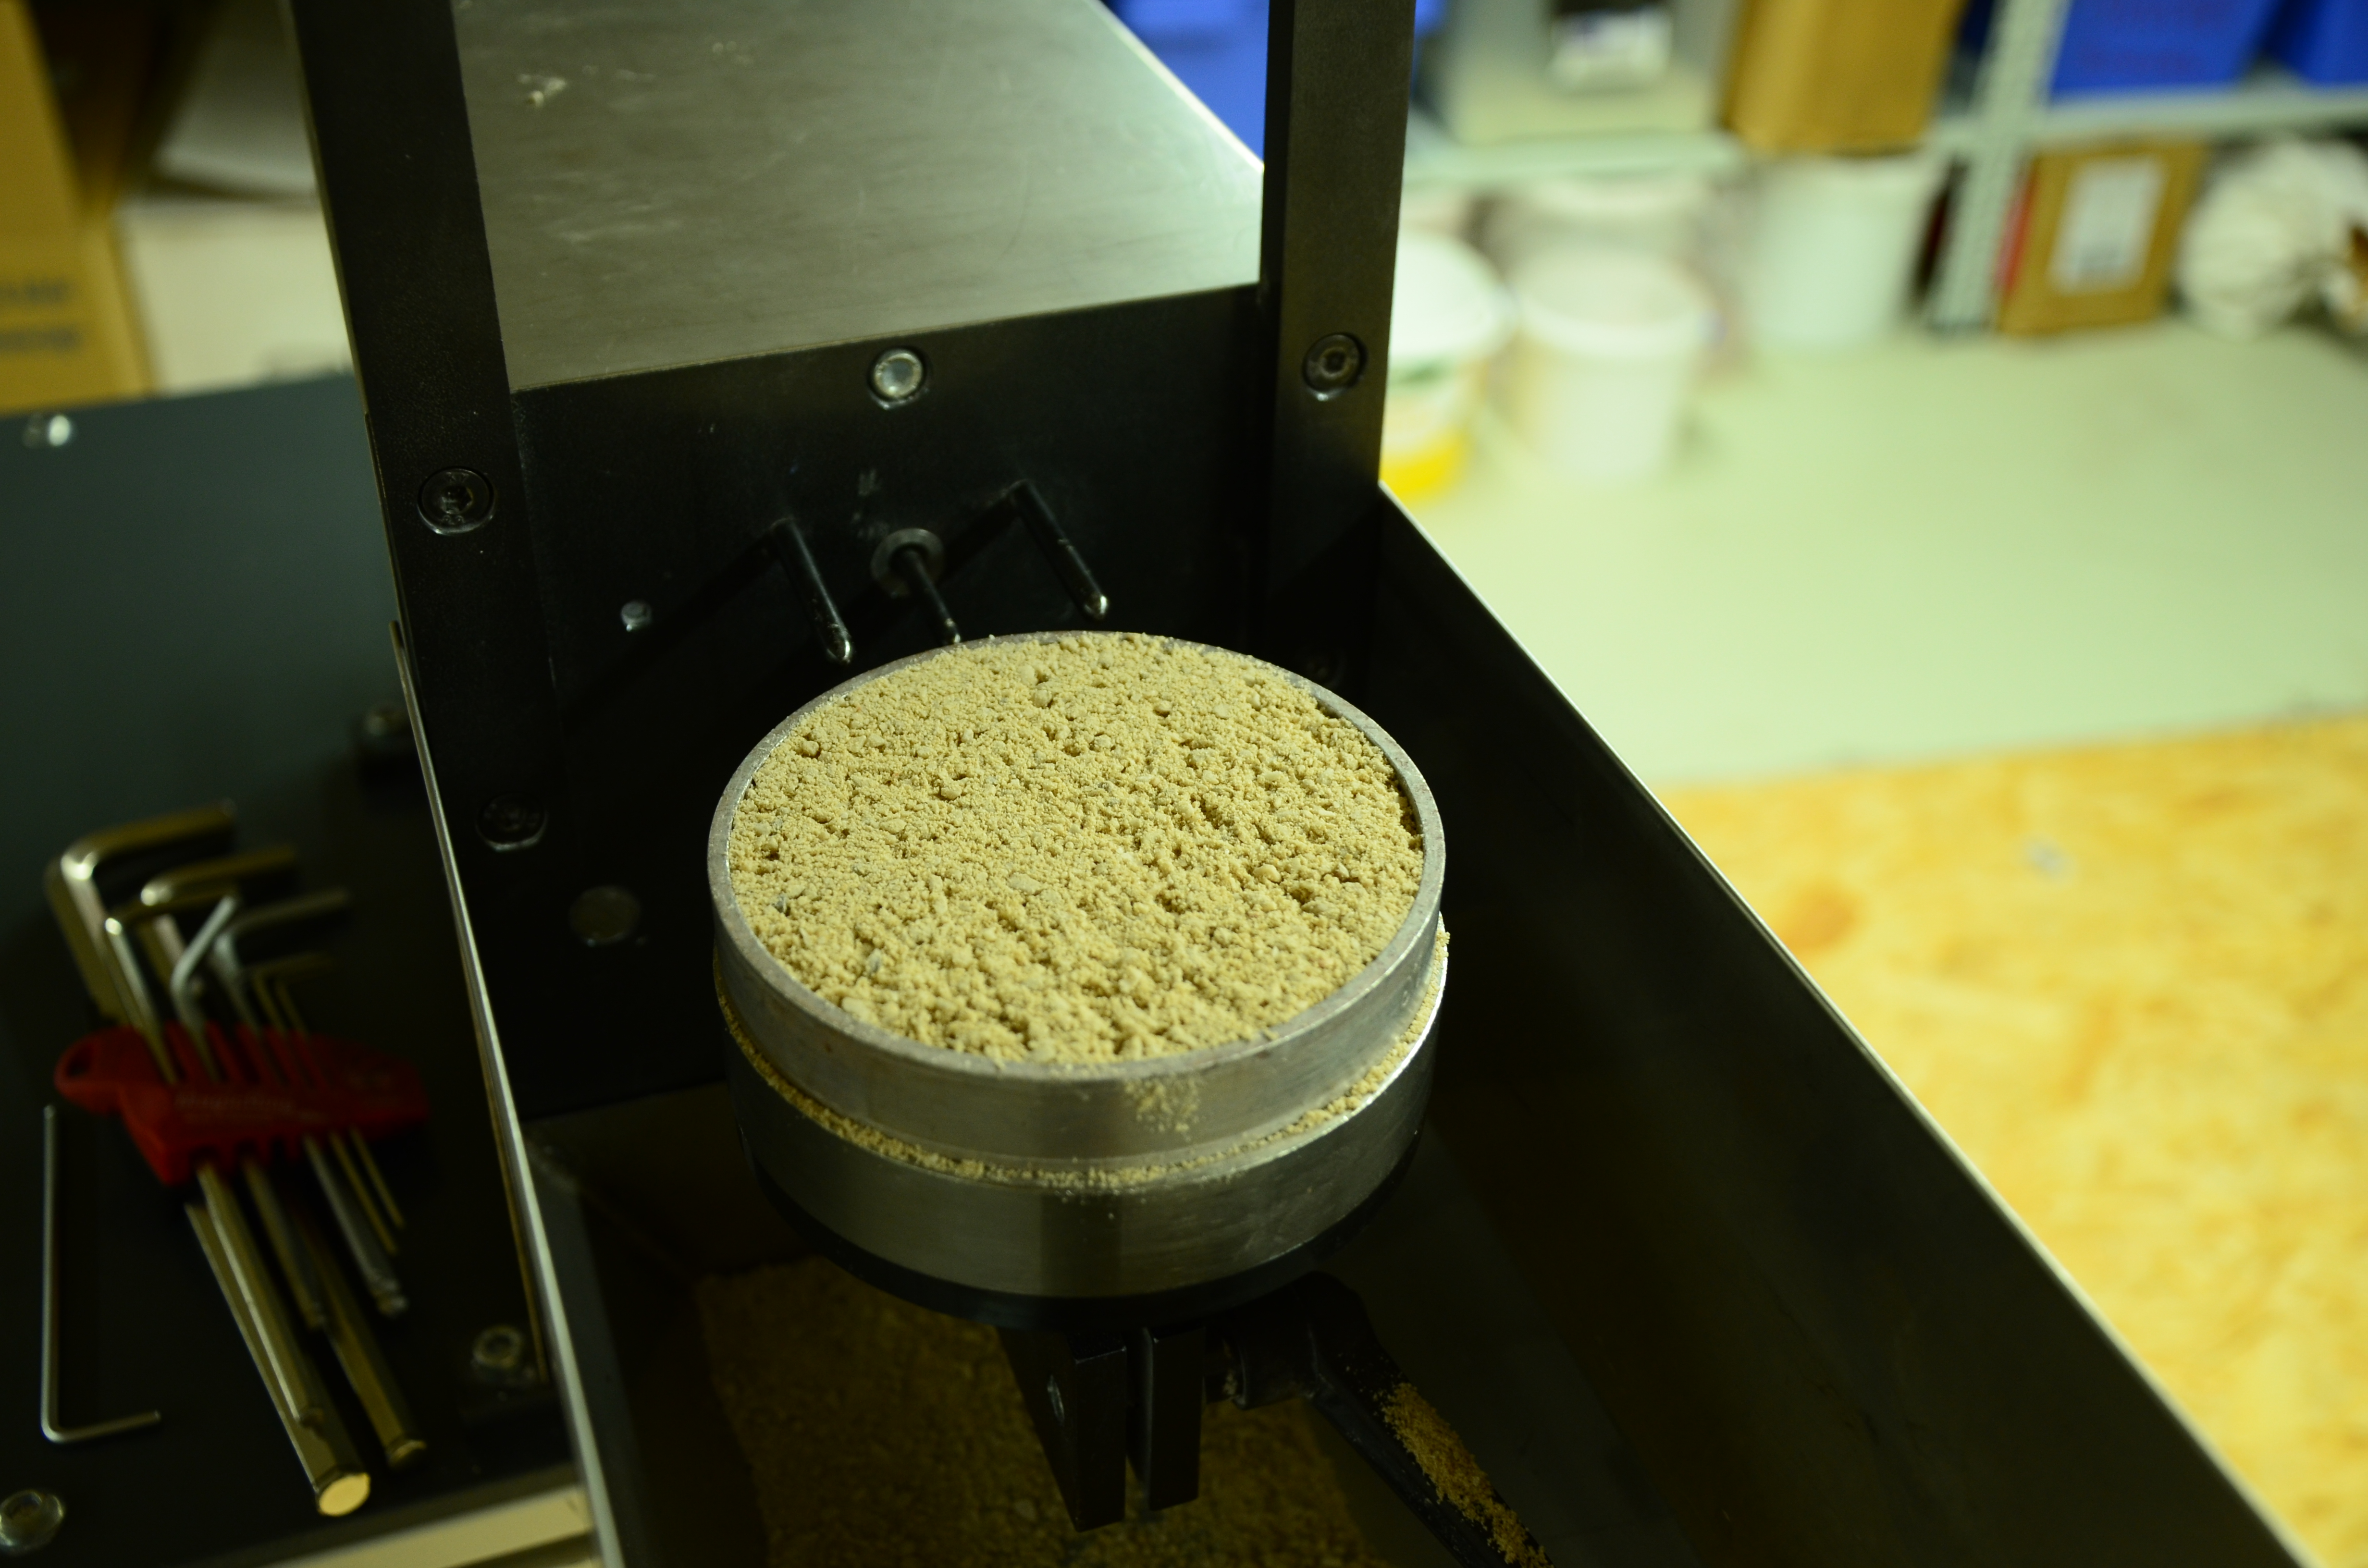
\includegraphics[width=.80\columnwidth]{images/052ShearCellLab}
\caption[JSCT]{Jenike shear cell tester.}
\label{fig:052ShearCellLab}
\end{figure}
\begin{figure}[!htb]
\centering
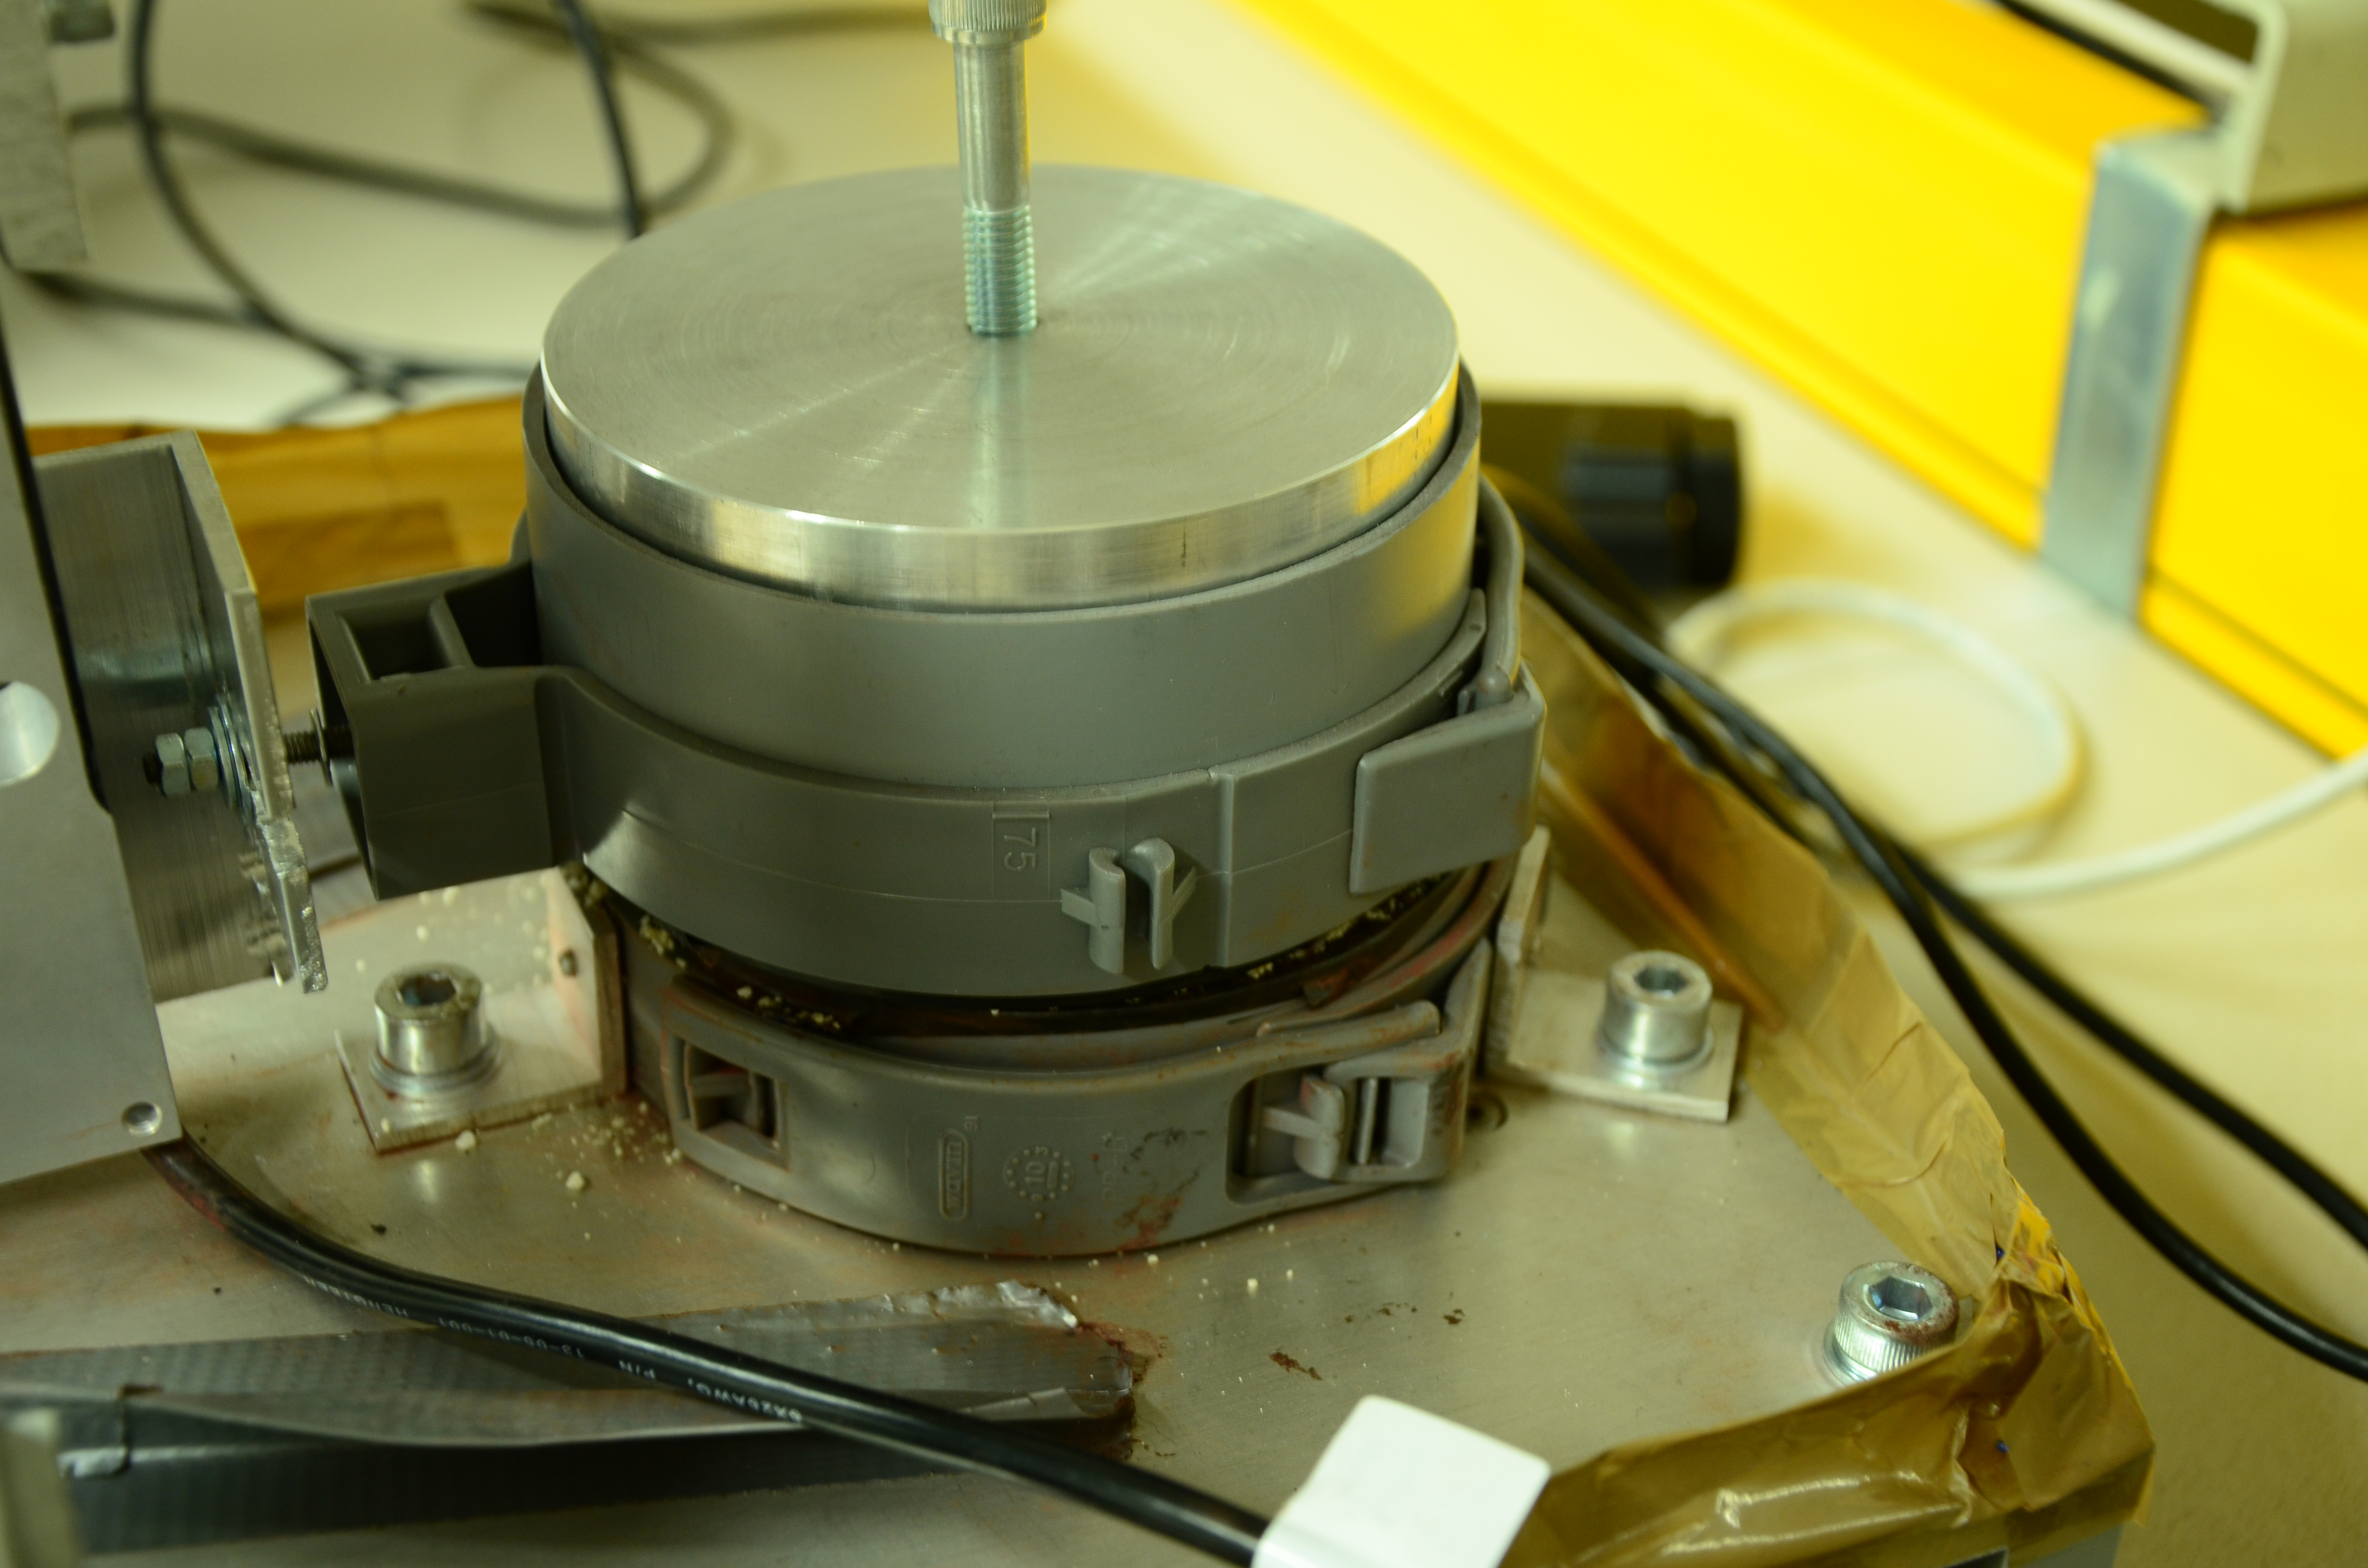
\includegraphics[width=.80\columnwidth]{images/053PoorMan}
\caption[SJSCT]{Laboratory setup of the simplified Jenike shear cell
tester.}
\label{fig:053PoorMan}
\end{figure}

Fig. \ref{fig:003sjsct} \\
\begin{figure}[!htb]
\centering
\includegraphics[width=.80\columnwidth]{images/003sjsct}
\caption[Jenike shear cell tester]{Jenike shear cell tester.}
\label{fig:003sjsct}
\end{figure}

Fig. \ref{fig:004sjsctdiagram} \\
\begin{figure}[!htb]
\centering
\includegraphics[width=.80\columnwidth]{images/004sjsctdiagram}
\caption[Jenike shear cell diagram]{Jenike shear cell diagram
\cite{RefWorks:69}.}
\label{fig:004sjsctdiagram}
\end{figure}

\section{Schulze Ring Shear Cell tester (p-p)}
\label{sec:SRSCT}
%************************************************

A representative sample of bulk solid was placed in a shear cell of specified
dimensions ($external ~ radius = 100 ~ mm$, $internal ~ radius = 50 ~ mm$).
A normal load was applied to the cover. As soon as the lid touched the sample,
its position was calculated.
Together with the area of the ring, the total volume can be calculated, and subsequently the $bulk ~ density ~ (\rho_b)$ 
of the sample was obtained the first bulk value.
Then the specimen was pre-sheared until a steady-state shear value was reached.
The steady-state flow horizontal stress
is called steady-state flow/pre-shear stress.
If the normal stress is known, it provides (Eq. \ref{eq:phi_ps}) the angle of
internal friction of the pre-shear phase ($\phi_{e-psh}$), and consequently the
pre-shear coefficient of internal friction $ (\mu_{psh})$, the second
bulk value, see Schulze \cite{RefWorks:118}:
%************************************************
\begin{equation}
\begin{aligned}
\phi_{e-psh} &= \arctan \left(\frac{\tau_{psh}}{\sigma_{n,psh}} \right) ,\\
\mu_{psh} &=\tan(\phi_{e-psh}) .
\end{aligned}
 \label{eq:phi_ps}
\end{equation}

%************************************************
The normal stress and the angular velocity were then immediately reduced to zero. 
Subsequently, the specimen was sheared under a fraction ($shear-perc$) of the first normal load until the shear force 
reached a maximum and began to decrease. 
Both the pre-shear and shear phases were executed at constant velocity. 
We define the horizontal stress at the shear force peak as the maximum shear
stress, thus obtaining the incipient flow/shear coefficient of internal friction $
(\mu_{sh})$, third bulk value (Eq. \ref{eq:phi_s})\cite{RefWorks:118}:
%************************************************
\begin{equation}
\begin{aligned}
\phi_{e-sh} &= \arctan \left(\frac{\tau_{sh}}{\sigma_{n,sh}} \right) ,\\
\mu_{sh} &= \tan(\phi_{e-sh}) .
\end{aligned}
 \label{eq:phi_s}
\end{equation}

%************************************************
Three different pre-shear normal loads were applied in the experiment
(1,000, 2,000, and 10,000 Pa).
For each we used a normal load proportional to the initial one
(\textit{shear-perc}), increasing from stage one (40\%) to stage four (100\%)
with two escalating intermediate stages (60\% and 80\%) for a total of twelve load conditions.
Each experiment was performed on a fresh material sample. \\

\ref{fig:001srsct}.\\
\begin{figure}[!htb]
\centering
\includegraphics[width=.80\columnwidth]{images/001srsct}
\caption[Schulze ring shear cell tester]{Schulze ring shear cell tester.}
\label{fig:001srsct}
\end{figure}

\ref{fig:002srsctdiagram}.\\
\begin{figure}[!htb]
\centering
\includegraphics[width=.80\columnwidth]{images/002srsctdiagram}
\caption[Ring shear cell diagram]{Ring shear cell diagram \cite{RefWorks:69}.}
\label{fig:002srsctdiagram}
\end{figure}

\ref{fig:020experimental}.\\
\begin{figure}[!htb] 
\centering 
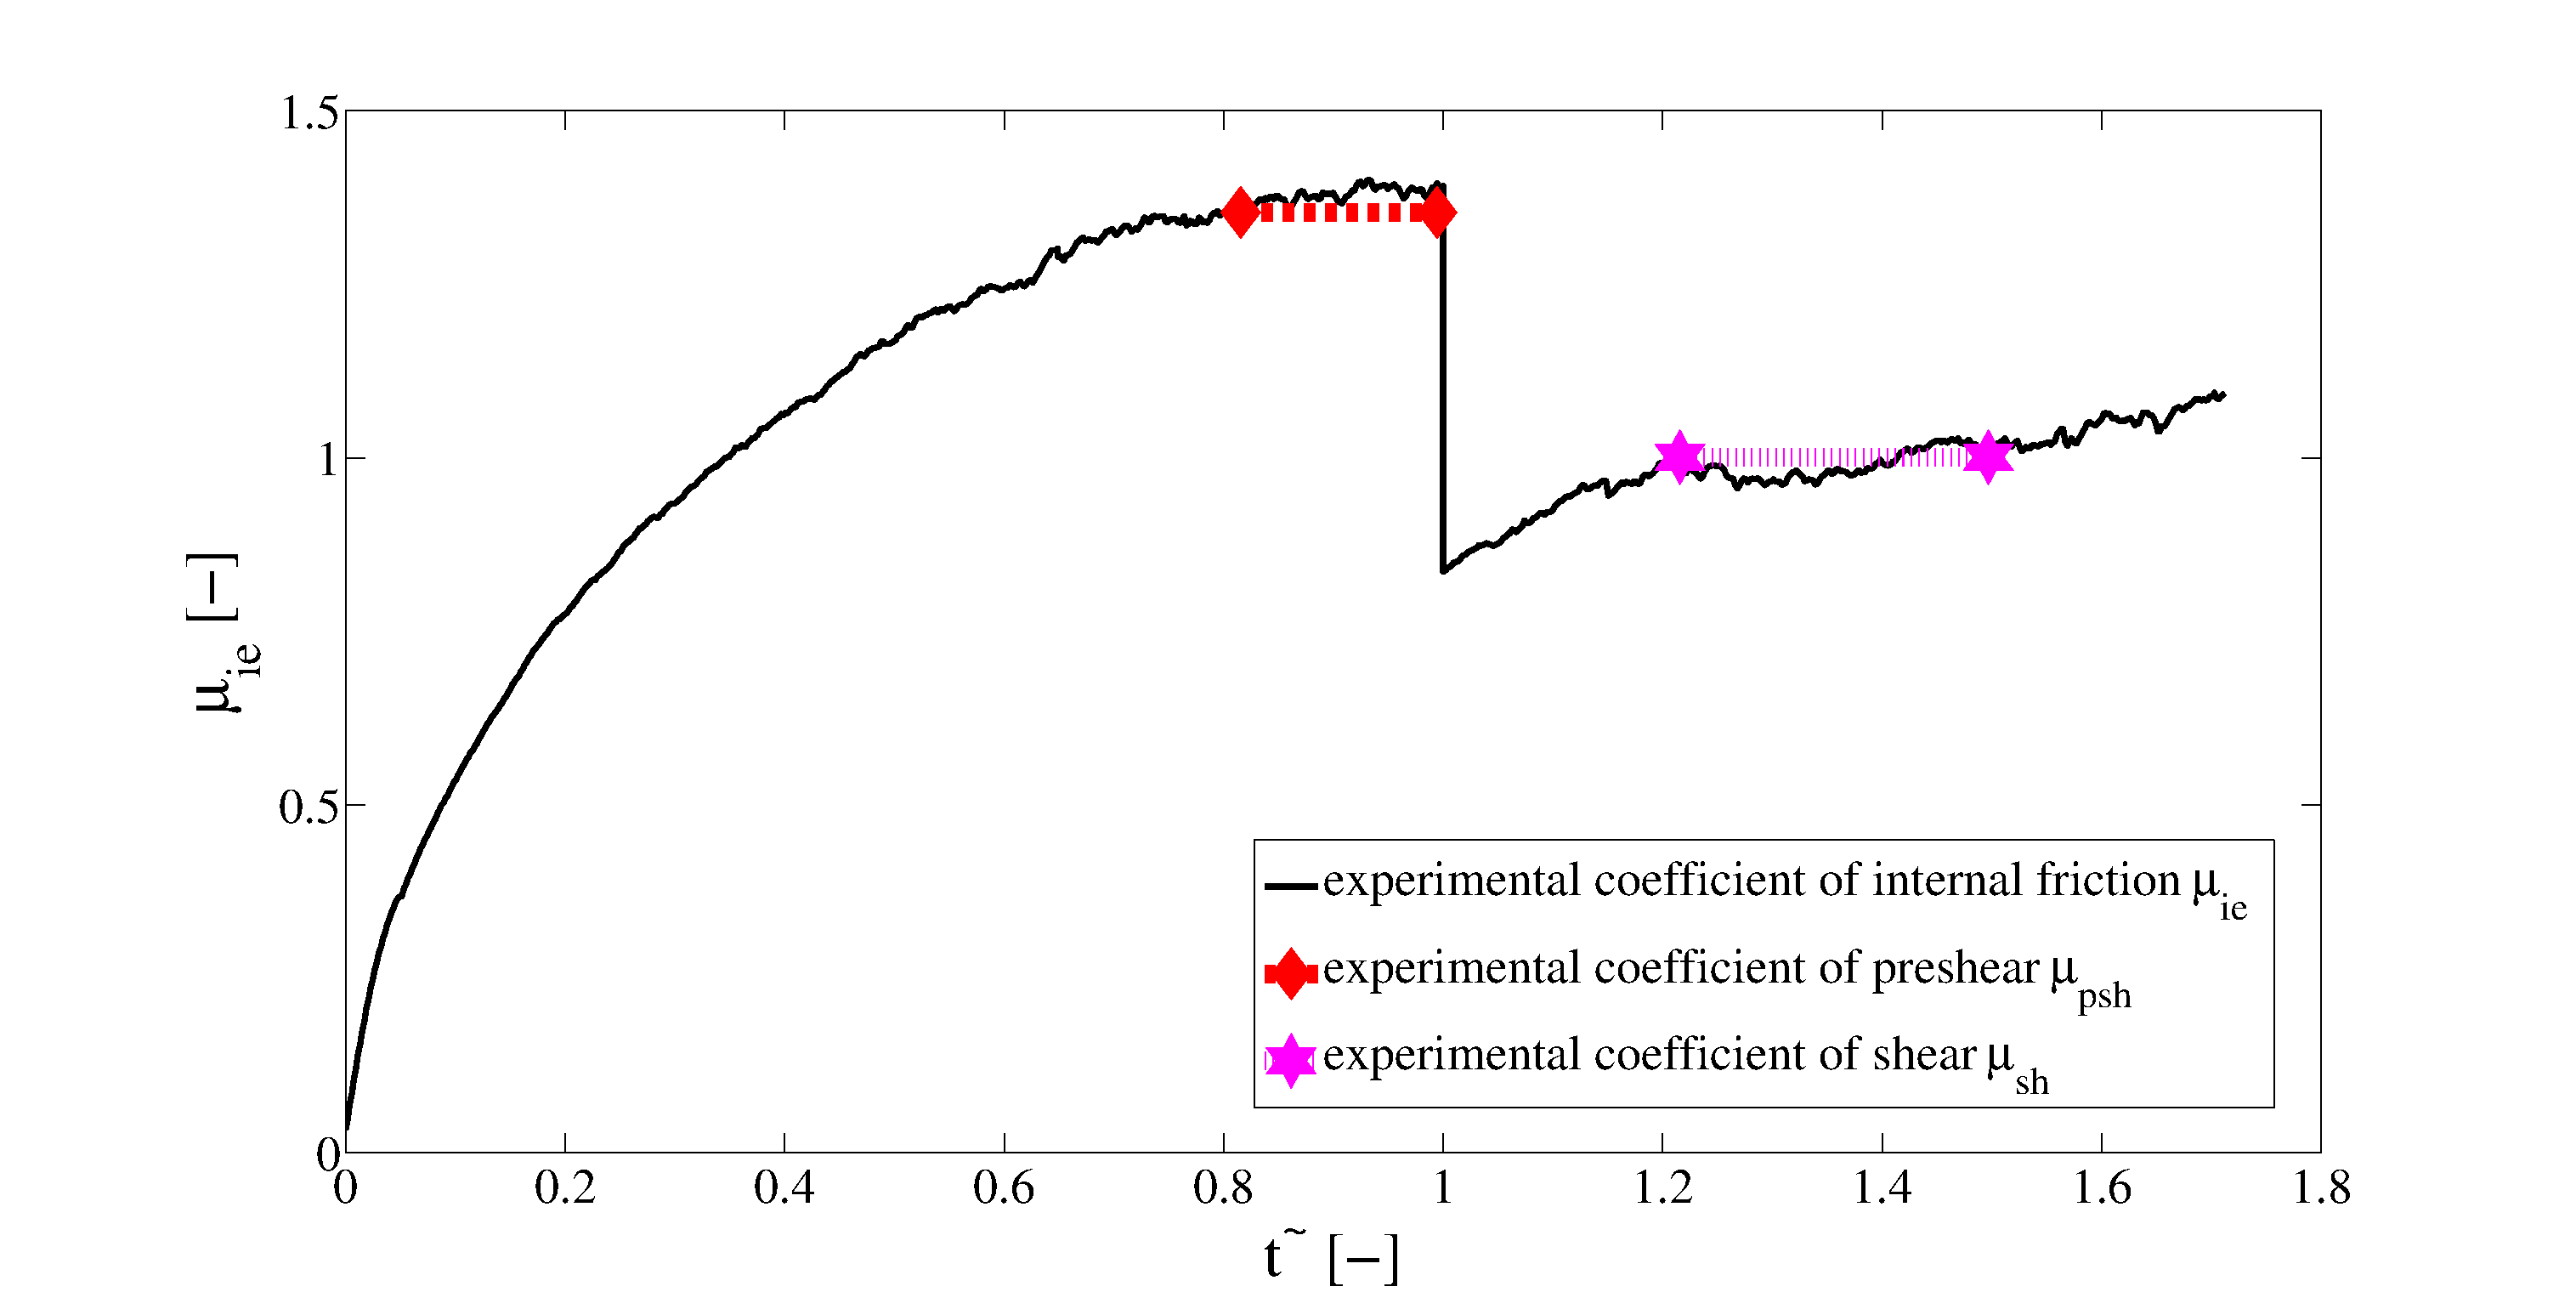
\includegraphics[width=.96\textwidth]{images/020experimental} 
\caption[Experimental shear cell tester stress path]{Experimental shear-cell tester stress path - $\sigma_n = 10000
        ~Pa$.}
\label{fig:020experimental} 
\end{figure}

% \begin{figure}[htp] \centering
%     \begin{subfigure}[b]{0.96\columnwidth}
%         \includegraphics[width=\textwidth]{20experimental}
%         \caption{Experimental shear-cell tester stress path - $\sigma_n = 10000
%         ~Pa$}
%         \label{fig:20experimental} 
%     \end{subfigure}\\
%         \begin{subfigure}[b]{0.96\columnwidth}
%         \includegraphics[width=\textwidth]{21simexample}
%         \caption{Numerical shear-cell tester stress path - $\sigma_n = 10000
%         ~Pa$}
%         \label{fig:21simexample} 
%     \end{subfigure}
%     \caption[Stress path]{Experimental and numerical samples of the stress path
%     for the Schulze ring shear cell tester.
% 	Time was normalized: $\tilde{t} = t/t_{change}$, where $t_{change}$ is the
% 	point in time at which the normal stress ($\sigma_n$) was modified during the
% 	tests.
% 	Until $\tilde{t}=1$, the $\sigma_n$ was kept constant at 10,000 Pa. 
% 	In Fig. \ref{fig:20experimental}, 
%  	a plateau was reached at $\tilde{t}~=0.91$.
% 	The coefficient of pre-shear ($\mu_{psh}$) was calculated as the average of the
% 	coefficient of internal friction ($\mu_{ie}$) in this first plateau.
% 	At $\tilde{t}=1$, the $\sigma_n$ was reduced to $80 \%$ of its initial
% 	value, and soon after
% 	a second plateau developed.
% 	We obtained the coefficient of
% 	shear ($ \mu_{sh}$) as the average of $\mu_{ie}$ in this second plateau.
% 	The stress paths agree well, especially the plateaux.
% 	They were clearly relevant because
% 	the values representative of the bulk behaviours 
% 	were collected there.}
%     \label{fig:40experimentalsimulation}
% \end{figure}

Experimental and numerical samples of the stress path
    for the Schulze ring shear cell tester.
	Time was normalized: $\tilde{t} = t/t_{change}$, where $t_{change}$ is the
	point in time at which the normal stress ($\sigma_n$) was modified during the
	tests.
	Until $\tilde{t}=1$, the $\sigma_n$ was kept constant at 10,000 Pa. 
	In Fig. \ref{fig:020experimental}, 
 	a plateau was reached at $\tilde{t}~=0.91$.
	The coefficient of pre-shear (\ac{mupsh}) was calculated as the average of the
	coefficient of internal friction ($\mu_{ie}$) in this first plateau.
	At $\tilde{t}=1$, the $\sigma_n$ was reduced to $80 \%$ of its initial
	value, and soon after
	a second plateau developed.
	We obtained the coefficient of
	shear ($ \mu_{sh}$) as the average of $\mu_{ie}$ in this second plateau.
	The stress paths agree well, especially the plateaux.
	They were clearly relevant because
	the values representative of the bulk behaviours 
	were collected there.










\section{Parameter Identification}
\label{sec:parameteridentification}

We obtained for each of the twelve load conditions of the $SSC$ three bulk
values (\ac{mupsh}, \ac{mush} and \ac{rhob}).
The fourth bulk value was the result of two angle of repose (\ac{AoR}) tests that
recreated the repose angle observed in a pile of the
real material. 

Subsequently, we compared the $ANN$ and experimental bulk behaviours for the
twelve shear-cell load conditions.
If in a DEM-parameter combination all the three bulk values differed by less 
than 5\% from those of the corresponding experiments, i.e.:
%************************************************
 \begin{equation}
 \begin{cases}
\text{if } & \lvert{1-\frac{\mu_{psh,num}}{\mu_{psh,exp}}}\rvert < 5\%  ,\\
\text{and if } & \lvert{1-\frac{\mu_{sh,num}}{\mu_{sh,exp}}}\rvert < 5\% , \\ 
\text{and if } & \lvert{1-\frac{\rho_{p,num}}{\rho_{p,exp}}}\rvert < 5\% ,\\ 
\end{cases}
 \label{eq:check2}
\end{equation}

the combination was marked. The marked combinations were processed by the
\ac{AoR} $ANN$, and then compared with the experiment.
Were considered valid those that differed by less than $5\%$ also in this
comparison (Eq. \ref{eq:checkaor}):
%************************************************
\begin{equation}
\text{if} ~~~~~~ \lvert{1-\frac{AoR_{num}}{AoR_{exp}}}\rvert < 5\% .
\label{eq:checkaor}
\end{equation}
%************************************************
Further, to prove the validity of the system, we tested the marked combinations
by modifying the experimental bulk values of the shear cell. 
We artificially decreased or increased the shear force, and thus \ac{mupsh} and
\ac{mush}, by a product coefficient ($P$), e.g. Eq. \ref{eq:pcoeff}:
%************************************************
\begin{equation}
\label{eq:pcoeff}
\mu_{psh, new} = \mu_{psh, old} \cdot P .
\end{equation}
%************************************************